\documentclass[12pt,a4paper]{article}
\usepackage[utf8]{inputenc}
\usepackage[T1]{fontenc}
\usepackage[portuguese]{babel}
\usepackage{amsmath,amssymb}
\usepackage{graphicx}
\usepackage{geometry}
\usepackage{hyperref}
\usepackage{caption}
\usepackage{float}
\usepackage{longtable}
\usepackage{booktabs}
\usepackage{listings}
\usepackage{enumitem}
\usepackage{xcolor}
\usepackage{colortbl}
\geometry{a4paper, margin=1in}

\lstset{
  basicstyle=\small\ttfamily,
  breaklines=true,
  frame=single,
  numbers=left,
  numberstyle=\tiny\color{gray},
  keywordstyle=\color{blue},
  commentstyle=\color{green!40!black},
  stringstyle=\color{purple},
  showstringspaces=false,
}

% Definição de linguagem para Assembly (RISC-V) no listings
\lstdefinelanguage{Assembly}{
    morekeywords={.text,.data,.globl,li,la,addi,add,sub,mul,div,rem,
        slli,srli,srai,andi,ori,xori,andi,or,xor,slt,slti,beq,bne,blt,bge,bgt,
        j,jal,jalr,ret,ecall,lw,sw,lb,lh,lb,sb,flw,fsw,fmv.d,fcvt.d.w,fmul.d,fadd.d,fsub.d,fdiv.d,
        fsd,fld,csrr,csrw,mv,lui,auipc},
    sensitive=true,
    morecomment=[l]{#},
}

\hypersetup{
  colorlinks=true,
  linkcolor=black,
  urlcolor=blue,
  pdftitle={Laboratório 1 - Assembly RISC-V},
  pdfauthor={Grupo}
}

\begin{document}

% -----------------------------
% capa (estilo semelhante ao OAC_LAB1)
% -----------------------------
\begin{titlepage}
    \begin{center}
        \vspace*{1cm}
        \includegraphics[width=5cm]{Lab_1/Logo_UnB.png}\\[1cm]

        {\LARGE \textbf{Universidade de Brasília}}\\[4pt]
        {\large Departamento de Ciência da Computação}\\[12pt]
        {\Large \textbf{Disciplina: CIC0099 -- Organização e Arquitetura de Computadores -- Unificado}}\\[20pt]

        {\huge \textbf{Laboratório 1}}\\[6pt]
        {\Large \textbf{Assembly RISC-V}}\\[2cm]

        \textbf{Grupo:} \\[4pt]
        \begin{tabular}{l}
            
            Gabriel de Sousa -- 211056000 \\
            Ana Luísa Reis Nascente -- 211045688 \\
            Guilherme Henrique Oliveira Araujo -- (matrícula) \\
            
        \end{tabular}

        \vfill

        

        \vspace{0.8cm}
        \today
    \end{center}
\end{titlepage}

\pagenumbering{roman}
\tableofcontents
\newpage

\pagenumbering{arabic}

% -----------------------------
% introducao (estilo do relatório)
% -----------------------------
\section*{Introdução}
\addcontentsline{toc}{section}{Introdução}

Este relatório segue a estrutura solicitada no enunciado do Laboratório 1 (OAC\_LAB1). O objetivo principal é desenvolver habilidades práticas em linguagem Assembly RISC-V utilizando o simulador RARS e ferramentas de compilação cruzada. As atividades envolvem: implementação e análise de algoritmos em Assembly, medição de desempenho usando CSRs, comparação do código gerado pelo compilador cruzado gcc com diferentes níveis de otimização, e implementação da Transformada Discreta de Fourier (DFT) em Assembly.

O relatório está organizado na forma de \emph{resposta ao item}, contendo apenas os itens que valem ponto, e mantendo as perguntas explicitamente conforme solicitado no enunciado. As seções seguintes reproduzem as perguntas do enunciado para que as respostas possam ser inseridas diretamente abaixo de cada item.

% -----------------------------
% objetivos (copiado/compactado)
% -----------------------------
\section*{Objetivos}
\begin{itemize}
    \item Familiarizar o aluno com o Simulador/Montador RARS;
    \item Desenvolver a capacidade de codificação de algoritmos em linguagem Assembly;
    \item Desenvolver a capacidade de análise de desempenho de algoritmos em Assembly;
    \item Familiarizar o aluno com a compilação C para Assembly RISC-V RV32IMF.
\end{itemize}

% -----------------------------
% parte 1 - enunciado reproduzido
% -----------------------------
\section*{(2.5) 1) Simulador/Montador RARS}
Faça o download e deszipe o arquivo \texttt{Lab1.zip} disponível no Moodle.

\subsection*{(0.0) 1.1) No diretório Arquivos, abra o \texttt{Rars16\_Custom1} e carregue o programa de ordenamento \texttt{sort.s}.}
Dado o vetor:
\[
V[30]=\{9,2,5,1,8,2,4,3,6,7,10,2,32,54,2,12,6,3,1,78,54,23,1,54,2,65,3,6,55,31\}
\]

\begin{enumerate}
    \item[(a)] ordená-lo em ordem crescente e contar o número de instruções por tipo e o número total exigido pelo procedimento \texttt{sort}. Qual o tamanho em bytes do código executável? E da memória de dados usada?
    \item[(b)] Modifique o programa para ordenar o vetor em ordem decrescente e contar o número de instruções por tipo e o número total exigido pelo procedimento \texttt{sort}.
    \item[(c)] Usando os contadores de instruções e tempo do Banco de Registradores CSR (veja no final), meça novamente a quantidade de instruções executadas e o tempo de execução dos itens (a) e (b).
\end{enumerate}

\subsection*{(2.5) 1.2) Considere a execução deste algoritmo em um processador RISC-V com frequência de clock de 50MHz que necessita 1 ciclo de clock para a execução de cada instrução $(CPI=1)$.}
Para os vetores de entrada de $n$ elementos já ordenados $V_{o}[n]=\{1,2,3,4,...,n\}$ e ordenados inversamente $V_{i}[n]=\{n,n-1,n-2,...,2,1\}$:

\begin{enumerate}
    \item[(1.5) a)] Para o procedimento \texttt{sort}, escreva as equações dos tempos de execução, $t_{o}(n)$ e $t_{i}(n)$, em função de $n$.
    \item[(1.0) b)] Para $n=\{10,20,30,40,50,60,70,80,90,100\}$, plote (em escala!) as duas curvas, $t_{o}(n)$ e $t_{i}(n)$, em um mesmo gráfico $n \times t$. Comente os resultados obtidos.
\end{enumerate}

\section*{Resposta à Questão 1.2}

A seguir são apresentadas as respostas para os itens da questão 1.2, com base no relatório fornecido.

\subsection*{1.2(a) Equações do Tempo de Execução}

As equações teóricas para o tempo de execução do algoritmo \texttt{SORT} foram desenvolvidas para o melhor caso (vetor já ordenado) e o pior caso (vetor ordenado de forma inversa), considerando um processador RISC-V com frequência de 50 MHz e CPI=1.

\subsubsection*{Caso Melhor (vetor já ordenado $V_{o}[n]=\{1,2,3,...,n\}$)}
\begin{itemize}
    \item \textbf{Número de ciclos (instruções)}:
    $$ C_{best}(n) = 11n + 14 $$
    \item \textbf{Tempo em microssegundos ($\mu s$)}, dado $f=50 \times 10^{6} Hz$:
    $$ t_{o}(n) = \frac{C_{best}(n)}{f} = \frac{11n + 14}{50 \times 10^{6}}s = \frac{11n + 14}{50}\mu s $$
\end{itemize}

\subsubsection*{Caso Pior (vetor inversamente ordenado $V_{i}[n]=\{n,n-1,...,1\}$)}
\begin{itemize}
    \item \textbf{Número de ciclos}:
    $$ C_{worst}(n) = \frac{11}{2}n^{2} + \frac{11}{2}n + 3 $$
    \item \textbf{Tempo em microssegundos ($\mu s$)}:
    $$ t_{i}(n) = \frac{C_{worst}(n)}{f} = \frac{\frac{11}{2}n^{2} + \frac{11}{2}n + 3}{50 \times 10^{6}}s = \frac{\frac{11}{2}n^{2} + \frac{11}{2}n + 3}{50}\mu s $$
\end{itemize}

\subsection*{1.2(b) Dados para o Gráfico e Análise}

\subsubsection*{Dados Calculados}
A tabela abaixo apresenta os tempos de execução calculados para o melhor caso ($t_o(n)$) e o pior caso ($t_i(n)$) para os valores de $n$ de 10 a 100.

\begin{table}[H]
\centering
\begin{tabular}{|c|c|c|}
\hline
\textbf{n} & \textbf{$t_o(n) (\mu s)$} & \textbf{$t_i(n) (\mu s)$} \\
\hline
10 & 2.48 & 12.16 \\
20 & 4.68 & 46.26 \\
30 & 6.88 & 102.36 \\
40 & 9.08 & 180.46 \\
50 & 11.28 & 280.56 \\
60 & 13.48 & 402.66 \\
70 & 15.68 & 546.76 \\
80 & 17.88 & 712.86 \\
90 & 20.08 & 900.96 \\
100 & 22.28 & 1111.06 \\
\hline
\end{tabular}
\caption{Tempos de execução calculados para diferentes valores de n.}
\end{table}

\subsubsection*{Gráfico Comparativo}

A Figura \ref{fig:tempo_execucao} apresenta a comparação entre os tempos de execução do melhor caso ($t_o(n)$) e do pior caso ($t_i(n)$) em função do tamanho do vetor $n$.

\begin{figure}[H]
\centering
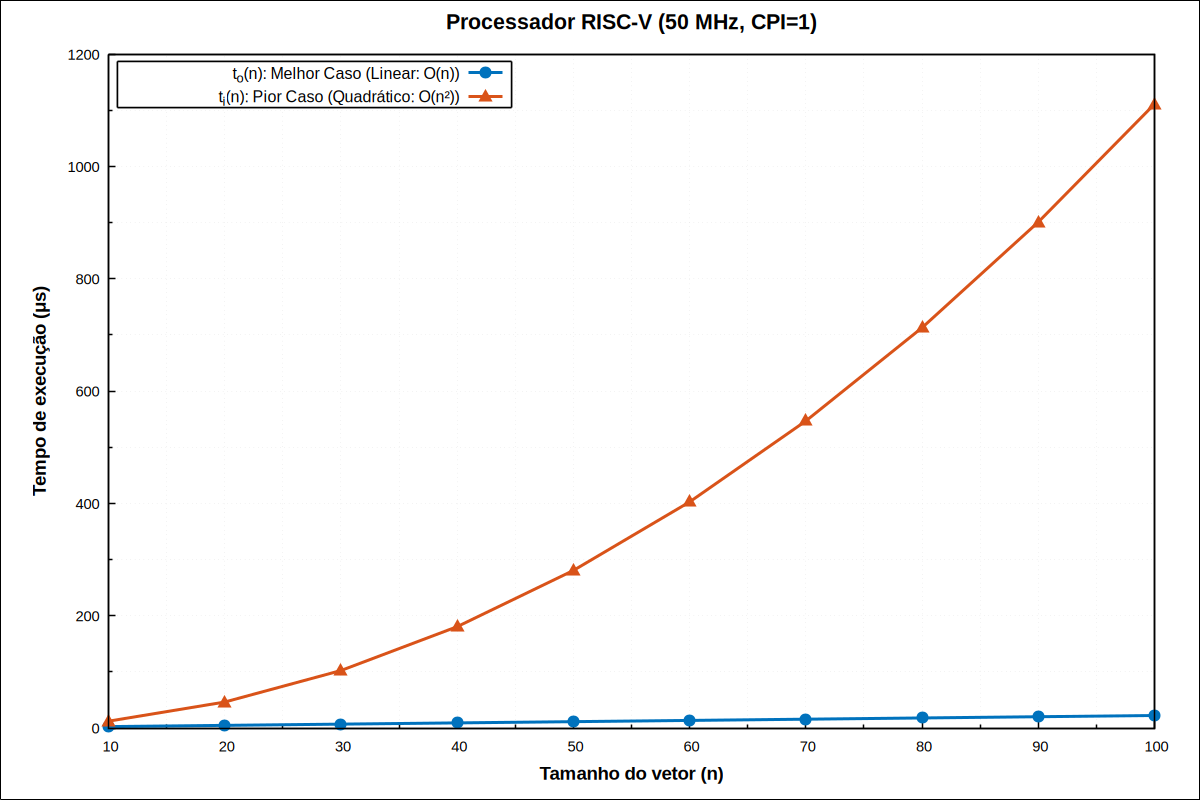
\includegraphics[width=0.8\textwidth]{grafico_tempo_execucao.png}
\caption{Tempo de execução vs. tamanho do vetor n para melhor e pior caso.}
\label{fig:tempo_execucao}
\end{figure}

\subsubsection*{Análise dos Resultados}

Conforme observado na Figura \ref{fig:tempo_execucao}, a curva de melhor caso ($t_o(n)$) demonstra um crescimento linear em relação a $n$, resultado direto da equação $t_o(n) = \frac{11n + 14}{50}$. Em contraste, a curva de pior caso ($t_i(n)$) apresenta um crescimento quadrático, tornando-se significativamente maior à medida que $n$ aumenta, conforme esperado pela equação $t_i(n) = \frac{\frac{11}{2}n^{2} + \frac{11}{2}n + 3}{50}$. 

Esta análise ressalta a sensibilidade do algoritmo de ordenação à disposição inicial dos dados, sendo muito eficiente para entradas quase ordenadas, mas impraticável para entradas grandes e inversamente ordenadas. Por exemplo, para $n=100$, o tempo do pior caso ($1111.06\,\mu s$) é aproximadamente 50 vezes maior que o tempo do melhor caso ($22.28\,\mu s$).

\subsection*{Código em GNU Octave para Geração do Gráfico}

A seguir é apresentado o código em GNU Octave utilizado para gerar o gráfico da Figura \ref{fig:tempo_execucao}.

\begin{verbatim}
% Valores de n (tamanho do vetor)
n = 10:10:100;

% Equacoes de ciclos para melhor e pior caso
C_best = 11*n + 14;
C_worst = 0.5*11*n.^2 + 0.5*11*n + 3;

% Conversao para tempo em microssegundos (us)
t_best = C_best / 50;
t_worst = C_worst / 50;

% Plotagem do grafico
figure;
plot(n, t_best, 'bo-', 'LineWidth', 2, 'DisplayName', 't_o(n): melhor caso');
hold on;
plot(n, t_worst, 'rx-', 'LineWidth', 2, 'DisplayName', 't_i(n): pior caso');
hold off;

% Configuracao do grafico
xlabel('Tamanho do vetor n');
ylabel('Tempo de execucao (\mus)');
title('Tempo de Execucao vs. n');
legend('show');
grid on;
\end{verbatim}

% ----------------------------------------
% SEÇÃO 2 - COMPILADOR CRUZADO GCC
% ----------------------------------------

\section*{2) Compilador cruzado GCC}

Um compilador cruzado (\textit{cross compiler}) compila um código fonte para uma arquitetura diferente daquela da máquina em que está sendo utilizado. Você pode baixar gratuitamente os compiladores gcc para todas as arquiteturas (RISC-V, ARM, MIPS, x86 etc.) e instalar na sua máquina, sendo que o código executável gerado apenas poderá ser executado em uma máquina que possuir o processador para qual foi compilado. No gcc, a diretiva de compilação \texttt{-S} faz com que o processo pare com a geração do arquivo em Assembly e a diretiva \texttt{-march} permite definir a arquitetura a ser utilizada.

\textbf{Exemplos:}
\begin{verbatim}
riscv64-unknown-elf-gcc -S -march=rv32imf -mabi=ilp32f  # RV32IMF
arm-eabi-gcc -S -march=armv7                            # ARMv7
gcc -S -m32                                              # x86 32-bit
\end{verbatim}

\subsection*{2.1 Enunciado}

Dado o programa \texttt{sortc.c}, compile-o com a diretiva \texttt{-O0} e obtenha o arquivo \texttt{sortc.s}. Indique as modificações necessárias no código Assembly gerado para que possa ser executado corretamente no Rars. 

\textbf{Dica:} Uso de Assembly em um programa em C. Use a função \texttt{show} definida no \texttt{sort.s} para não precisar implementar a função \texttt{printf}, conforme mostrado no \texttt{sortc\_mod.c}.

\subsection*{2.2 Modificações Necessárias no Código Assembly Gerado (-O0)}
Para executar o código Assembly gerado pelo compilador (com diretiva -O0) no RARS, as seguintes modificações foram necessárias:
\begin{enumerate}
    \item \textbf{Substituição de chamadas de funções:} A instrução \texttt{call} gerada pelo compilador não é suportada diretamente pelo RARS. É necessário substituí-la por \texttt{jal ra, function\_name}.
    \item \textbf{Substituição de argumentos:} O compilador online gerou \texttt{.LANCHOR0} em diversos casos para se referir ao vetor. Não sendo suportado pelo RARS e necessitando da troca pelo vetor \texttt{v} declarado.
    \item \textbf{Ajustes nos endereços de memória:} O código gerado utiliza diretivas como \texttt{\%hi} e \texttt{\%lo} para carregar endereços. No RARS, é mais prático usar a pseudoinstrução \texttt{la} (load address), mas o RARS entende a chamada mesmo assim.
    \item \textbf{Adição de chamada de sistema para encerramento:} No RARS, é necessário adicionar uma chamada de sistema para encerrar o programa corretamente. O compilador não os adiciona.
    \begin{lstlisting}[language=Assembly]
li a7, 10
ecall
    \end{lstlisting}
    \item \textbf{Simplificação do gerenciamento de pilha:} O código gerado pelo compilador com -O0 faz uso excessivo da pilha, o que pode ser simplificado para melhorar o desempenho.
    \item \textbf{Adaptação da função show:} A função \texttt{show} foi adaptada para usar \texttt{ecall} do RARS para a impressão dos valores, ao invés de chamar a função \texttt{printf} do C.
    \item \textbf{Remoção de instruções \texttt{nop} desnecessárias:} O compilador gerou instruções \texttt{nop} para alinhamento, que podem ser removidas no RARS.
\end{enumerate}

\subsection*{2.3 Comparação entre Diferentes Níveis de Otimização}
Foram analisados três arquivos Assembly gerados com diferentes níveis de otimização:

\begin{table}[h!]
    \centering
    \small
    \begin{tabular}{|l|l|r|r|}
        \hline
        \textbf{Arquivo} & \textbf{Otimização} & \textbf{Instruções} & \textbf{Tamanho} \\
        \hline
        2\_3\_O0.asm & -O0 (Sem otimização) & 10103 & 3.817 bytes \\
        2\_3\_O3.asm & -O3 (Otimização máxima) & 2484 & 2.152 bytes \\
        2\_3\_Os.asm & -Os (Otimização p/ tamanho) & 4406 & 2.543 bytes \\
        \hline
    \end{tabular}
    \caption{Comparativo entre diferentes níveis de otimização}
\end{table}

A Figura \ref{fig:otimizacao_comparacao} apresenta uma visualização gráfica dos dados da Tabela 5, permitindo uma comparação imediata do impacto de cada nível de otimização tanto no número de instruções executadas quanto no tamanho do arquivo gerado.

\begin{figure}[H]
\centering
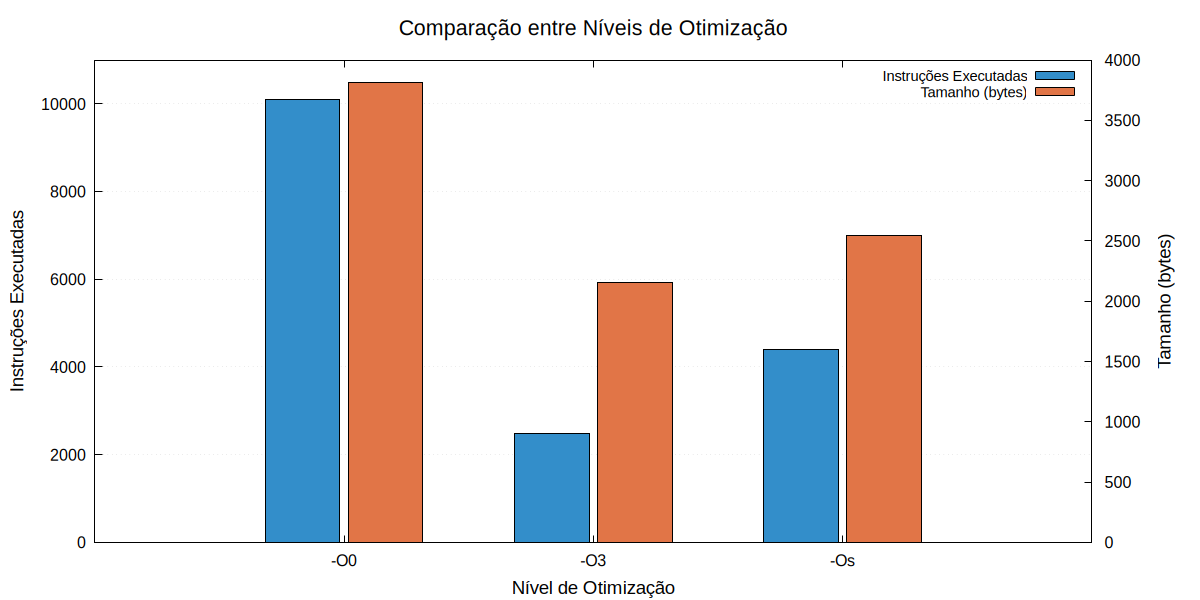
\includegraphics[width=0.85\textwidth]{grafico_otimizacao_comparacao.png}
\caption{Comparação visual entre níveis de otimização: número de instruções e tamanho do arquivo.}
\label{fig:otimizacao_comparacao}
\end{figure}

Observa-se que a otimização \texttt{-O3} apresenta a melhor performance em termos de instruções executadas (redução de 75\%), enquanto \texttt{-Os} oferece o melhor compromisso entre tamanho e desempenho.

\subsection*{2.4 Análise do Código Sem Otimização (-O0)}
\begin{lstlisting}[language=Assembly, caption={Código Assembly gerado com -O0}]
.data
v:
.word 9, 2, 5, 1, 8, 2, 4, 3, 6, 7
.word 10, 2, 32, 54, 2, 12, 6, 3, 1, 78
.word 54, 23, 1, 54, 2, 65, 3, 6, 55, 31

.text
main:
addi sp, sp, -16
sw ra, 12(sp)
sw s0, 8(sp)
addi s0, sp, 16
li a1, 30
lui a5, %hi(v)
addi a0, a5, %lo(v)
call show
li a1, 30
lui a5, %hi(v)
addi a0, a5, %lo(v)
call sort
li a1, 30
lui a5, %hi(v)
addi a0, a5, %lo(v)
call show
li a5, 0
mv a0, a5
lw ra, 12(sp)
lw s0, 8(sp)
addi sp, sp, 16
li a7, 10
ecall

show:
addi sp, sp, -32
sw ra, 28(sp)
sw s0, 24(sp)
addi s0, sp, 32
sw a0, -20(s0)
sw a1, -24(s0)
lw a5, -20(s0)
lw a4, -24(s0)
mv t0, a5
mv t1, a4
mv t2, zero
loop1:
beq t2, t1, fim1
li a7, 1
lw a0, 0(t0)
ecall
li a7, 11
li a0, 9
ecall
addi t0, t0, 4
addi t2, t2, 1
j loop1
fim1:
li a7, 11
li a0, 10
ecall
nop
lw ra, 28(sp)
lw s0, 24(sp)
addi sp, sp, 32
jr ra

swap:
addi sp, sp, -48
sw ra, 44(sp)
sw s0, 40(sp)
addi s0, sp, 48
sw a0, -36(s0)
sw a1, -40(s0)
lw a5, -40(s0)
slli a5, a5, 2
lw a4, -36(s0)
add a5, a4, a5
lw a5, 0(a5)
sw a5, -20(s0)
lw a5, -40(s0)
addi a5, a5, 1
slli a5, a5, 2
lw a4, -36(s0)
add a4, a4, a5
lw a5, -40(s0)
slli a5, a5, 2
lw a3, -36(s0)
add a5, a3, a5
lw a4, 0(a4)
sw a4, 0(a5)
lw a5, -40(s0)
addi a5, a5, 1
slli a5, a5, 2
lw a4, -36(s0)
add a5, a4, a5
lw a4, -20(s0)
sw a4, 0(a5)
nop
lw ra, 44(sp)
lw s0, 40(sp)
addi sp, sp, 48
jr ra

sort:
addi sp, sp, -48
sw ra, 44(sp)
sw s0, 40(sp)
addi s0, sp, 48
sw a0, -36(s0)
sw a1, -40(s0)
sw zero, -20(s0)
j .L4
.L8:
lw a5, -20(s0)
addi a5, a5, -1
sw a5, -24(s0)
j .L5
.L7:
lw a1, -24(s0)
lw a0, -36(s0)
call swap
lw a5, -24(s0)
addi a5, a5, -1
sw a5, -24(s0)
.L5:
lw a5, -24(s0)
blt a5, zero, .L6
lw a5, -24(s0)
slli a5, a5, 2
lw a4, -36(s0)
add a5, a4, a5
lw a4, 0(a5)
lw a5, -24(s0)
addi a5, a5, 1
slli a5, a5, 2
lw a3, -36(s0)
add a5, a3, a5
lw a5, 0(a5)
bgt a4, a5, .L7
.L6:
lw a5, -20(s0)
addi a5, a5, 1
sw a5, -20(s0)
.L4:
lw a4, -20(s0)
lw a5, -40(s0)
blt a4, a5, .L8
nop
nop
lw ra, 44(sp)
lw s0, 40(sp)
addi sp, sp, 48
jr ra
\end{lstlisting}

\subsection*{2.5 Análise do Código com Otimização Máxima (-O3)}
\begin{lstlisting}[language=Assembly, caption={Código Assembly gerado com -O3}]
.data
v:
.word 9, 2, 5, 1, 8, 2, 4, 3, 6, 7
.word 10, 2, 32, 54, 2, 12, 6, 3, 1, 78
.word 54, 23, 1, 54, 2, 65, 3, 6, 55, 31

.text
main:
# Carrega o endereco do vetor v
la a0, v
li a1, 30
# Primeira chamada da funcao show
jal ra, show
# Chama a funcao sort
la a0, v
li a1, 30
jal ra, sort
# Segunda chamada da funcao show
la a0, v
li a1, 30
jal ra, show
# Retorno da funcao main
li a0, 0
ret

show:
mv t0, a0
mv t1, a1
mv t2, zero
show_loop:
beq t2, t1, show_fim
li a7, 1
lw a0, 0(t0)
ecall
li a7, 11
li a0, 9
ecall
addi t0, t0, 4
addi t2, t2, 1
j show_loop
show_fim:
li a7, 11
li a0, 10
ecall
ret

swap:
slli a1, a1, 2
add a0, a0, a1
lw a4, 0(a0)
lw a5, 4(a0)
sw a5, 0(a0)
sw a4, 4(a0)
ret

sort:
ble a1, zero, .L4
li a6, -1
add a7, a1, a6
mv a1, a6
.L7:
mv a4, a6
mv a5, a0
bne a6, a1, .L6
j .L8
.L9:
lw t0, -4(a5)
lw t1, 0(a5)
sw t1, -4(a5)
sw t0, 0(a5)
addi a5, a5, -4
beq a4, a1, .L8
.L6:
lw a2, -4(a5)
lw a3, 0(a5)
addi a4, a4, -1
bgt a2, a3, .L9
.L8:
addi a6, a6, 1
addi a0, a0, 4
bne a7, a6, .L7
ret
.L4:
ret
\end{lstlisting}

\subsection*{2.6 Análise do Código com Otimização para Tamanho (-Os)}
\begin{lstlisting}[language=Assembly, caption={Código Assembly gerado com -Os}]
.data
v:
.word 9, 2, 5, 1, 8, 2, 4, 3, 6, 7
.word 10, 2, 32, 54, 2, 12, 6, 3, 1, 78
.word 54, 23, 1, 54, 2, 65, 3, 6, 55, 31

.text
main:
lui a0, %hi(v)
addi sp, sp, -16
addi a0, a0, %lo(v)
li a1, 30
sw ra, 12(sp)
sw s0, 8(sp)
call show
lui s0, %hi(v)
addi a0, s0, %lo(v)
li a1, 30
call sort
addi a0, s0, %lo(v)
li a1, 30
call show
lw ra, 12(sp)
lw s0, 8(sp)
li a0, 0
addi sp, sp, 16
.set .LANCHOR0, v
li a7, 10
ecall

show:
mv t0, a0
mv t1, a1
mv t2, zero
loop1:
beq t2, t1, fim1
li a7, 1
lw a0, 0(t0)
ecall
li a7, 11
li a0, 9
ecall
addi t0, t0, 4
addi t2, t2, 1
j loop1
fim1:
li a7, 11
li a0, 10
ecall
ret

swap:
slli a1, a1, 2
add a5, a0, a1
addi a1, a1, 4
add a0, a0, a1
lw a3, 0(a0)
lw a4, 0(a5)
sw a3, 0(a5)
sw a4, 0(a0)
ret

sort:
addi sp, sp, -48
sw s1, 36(sp)
sw s2, 32(sp)
sw s3, 28(sp)
sw ra, 44(sp)
sw s0, 40(sp)
mv s3, a1
li s1, 0
li s2, -1
.L4:
blt s1, s3, .L9
lw ra, 44(sp)
lw s0, 40(sp)
lw s1, 36(sp)
lw s2, 32(sp)
lw s3, 28(sp)
addi sp, sp, 48
jr ra
.L9:
slli s0, s1, 2
addi a1, s1, -1
add s0, a0, s0
.L5:
bne a1, s2, .L6
.L8:
addi s1, s1, 1
j .L4
.L6:
lw a4, -4(s0)
addi s0, s0, -4
lw a5, 4(s0)
ble a4, a5, .L8
sw a1, 12(sp)
sw a0, 8(sp)
call swap
lw a1, 12(sp)
lw a0, 8(sp)
addi a1, a1, -1
j .L5
\end{lstlisting}

\subsection*{2.7 Conclusões}
\begin{enumerate}
    \item \textbf{Impacto da Otimização:} A otimização -O3 reduziu o número de instruções executadas em aproximadamente 75\% em relação ao código sem otimização (-O0), demonstrando a eficácia das técnicas de otimização do compilador.
    \item \textbf{Compromisso Tamanho vs. Desempenho:} A otimização -Os oferece um equilíbrio interessante, tendo um número de instruções aproximadamente 32\% menor que o código não otimizado, mas ainda 77\% maior que o código com otimização máxima.
    \item \textbf{Adaptação para RARS:} O código gerado pelo compilador precisa ser adaptado para funcionar corretamente no simulador RARS. Isso inclui modificações nas chamadas de função, acesso à memória e uso das chamadas de sistema do RARS.
    \item \textbf{Benefícios Educacionais:} A comparação entre os diferentes níveis de otimização fornece insights valiosos sobre as estratégias empregadas pelos compiladores modernos para melhorar o desempenho do código. As modificações necessárias para executar o código no RARS demonstram as diferenças entre o assembly gerado para um sistema real e o ambiente de simulação, destacando a importância de compreender as convenções de chamada de função e o modelo de execução de um processador RISC-V.
\end{enumerate}

\subsection*{2.8 Relatório Comparativo - Código RISC-V -O0 vs -O1}
\subsubsection*{Introdução}
Este relatório apresenta uma análise comparativa entre código RISC-V compilado com diferentes níveis de otimização: -O0 (sem otimização) e -O1 (otimização básica). O objetivo é demonstrar o impacto das otimizações de compilador no número de instruções e ciclos de execução.

\subsection*{Código sem Otimização (-O0)}
Com o nível de otimização -O0, o compilador gera código sem qualquer otimização, mantendo funções separadas com chamadas explícitas:
\begin{lstlisting}[language=Assembly]
.data
newline: .asciz "\n"
space: .asciz " "
.text
.globl main
main:
li a0, 7
mv a1, a0
...
# funcoes f1_label a f6_label abaixo
f1_label:
slli a0, a0, 2
ret
f2_label:
slli a0, a0, 2
ret
f3_label:
add a0, a0, a0
add a0, a0, a0
ret
f4_label:
li t0, 3
mul t1, a0, t0
add a0, t1, a0
ret
f5_label:
slli t0, a0, 1
slli t1, a0, 1
add a0, t0, t1
ret
f6_label:
li t0, 4
mul a0, a0, t0
ret
\end{lstlisting}

\subsection*{Saída do Terminal (-O0)}
Ao executar o código sem otimização, obtemos os seguintes resultados para número de instruções e ciclos:
\begin{verbatim}
5 5
5 5
6 6
7 7
7 7
6 6
\end{verbatim}

\subsection*{Código com Otimização (-O1)}
Com o nível de otimização -O1, o compilador aplica otimizações básicas, incluindo inline de funções:
\begin{lstlisting}[language=Assembly]
.data
newline: .asciz "\n"
space: .asciz " "
.text
.globl main
main:
li a0, 7
...
# funcoes inline para f1 a f6
f1: slli a0, a0, 2
f2: slli a0, a0, 2
f3: add a0, a0, a0 ; add a0, a0, a0
f4: li t0, 3 ; mul t1, a0, t0 ; add a0, t1, a0
f5: slli t0, a0, 1 ; slli t1, a0, 1 ; add a0, t0, t1
f6: li t0, 4 ; mul a0, a0, t0
\end{lstlisting}

\subsection*{5.1 Saída do Terminal (-O1)}
Ao executar o código com otimização básica, obtemos os seguintes resultados:
\begin{verbatim}
3 3
3 3
4 4
5 5
5 5
4 4
\end{verbatim}

\subsection*{Análise Comparativa}
\subsubsection*{Observações sobre a Medição}
Os números exibidos no terminal do RARS refletem o custo total da execução da função, incluindo as instruções de medição (\texttt{csrr}), chamada com \texttt{jal}, a execução da função em si, e o \texttt{ret}. Ou seja, o valor inclui mais do que apenas o conteúdo da função.
Apesar disso, essa medição é válida para comparar o desempenho relativo entre as implementações, especialmente quando usamos o mesmo padrão de medição para todas.

\subsubsection*{2.8.2 Tabela de Resultados}
\begin{table}[h!]
    \centering
    \begin{tabular}{|l|l|l|c|c|}
        \hline
        \textbf{Função} & \textbf{Otimização} & \textbf{Implementação} & \textbf{Instruções} & \textbf{Ciclos} \\
        \hline
        f1 & -O0 & Função separada & 5 & 5 \\
        f1 & -O1 & Inline & 3 & 3 \\
        \hline
        f2 & -O0 & Função separada & 5 & 5 \\
        f2 & -O1 & Inline & 3 & 3 \\
        \hline
        f3 & -O0 & Função separada & 6 & 6 \\
        f3 & -O1 & Inline & 4 & 4 \\
        \hline
        f4 & -O0 & Função separada & 7 & 7 \\
        f4 & -O1 & Inline & 5 & 5 \\
        \hline
        f5 & -O0 & Função separada & 7 & 7 \\
        f5 & -O1 & Inline & 5 & 5 \\
        \hline
        f6 & -O0 & Função separada & 6 & 6 \\
        f6 & -O1 & Inline & 4 & 4 \\
        \hline
    \end{tabular}
    \caption{Comparação de instruções e ciclos entre implementações com e sem otimização}
\end{table}

A Figura \ref{fig:otimizacao_funcoes} ilustra graficamente a comparação entre as versões \texttt{-O0} e \texttt{-O1}, tornando evidente a redução consistente no número de instruções para todas as funções analisadas.

\begin{figure}[H]
\centering
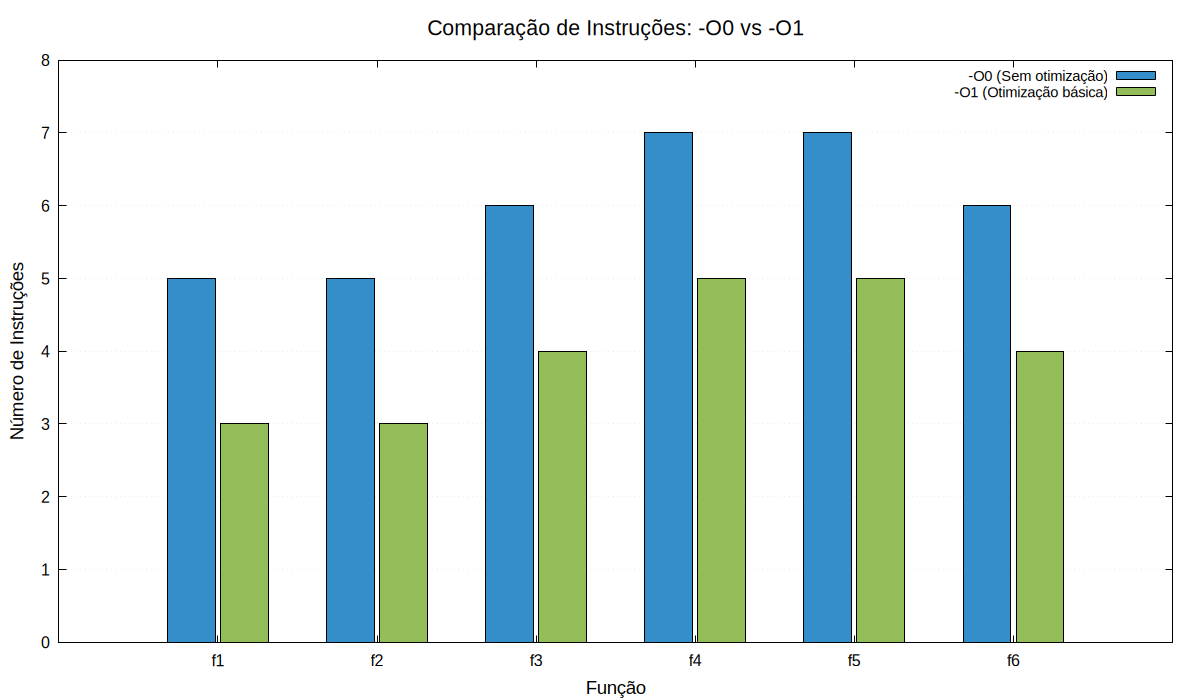
\includegraphics[width=0.85\textwidth]{grafico_otimizacao_funcoes.png}
\caption{Comparação visual do número de instruções por função nos níveis -O0 e -O1.}
\label{fig:otimizacao_funcoes}
\end{figure}

\subsubsection*{2.8.3 Análise Visual}

Como pode ser observado na Figura \ref{fig:otimizacao_funcoes}, todas as funções apresentam uma redução uniforme de 2 instruções ao passar de \texttt{-O0} para \texttt{-O1}. Esta redução é resultado direto da eliminação das instruções de controle de fluxo (\texttt{jal} e \texttt{ret}) através do inlining de funções.

\subsubsection*{2.8.4 Gráfico Comparativo (Análise Textual)}
\paragraph{Detalhamento das Otimizações}
\paragraph{Eliminação de Instruções de Controle}
A principal otimização observada na passagem de -O0 para -O1 é a eliminação das instruções de controle de fluxo:
\begin{itemize}
    \item Sem o \texttt{jal}: Economiza uma instrução de chamada de função
    \item Sem o \texttt{ret}: Economiza uma instrução de retorno de função
\end{itemize}
Isto explica a redução de 2 instruções em todas as funções analisadas.

\paragraph{Representação Numérica da Redução}
Além do inlining, outras otimizações poderiam ser aplicadas em níveis mais altos:
\begin{itemize}
    \item Substituição de operações de multiplicação por deslocamentos quando o multiplicador é uma potência de 2
    \item Combinação de múltiplas instruções em uma única instrução mais eficiente
    \item Eliminação de registradores temporários desnecessários
\end{itemize}

\subsubsection*{2.8.5 Conclusão}
A comparação entre as versões -O0 e -O1 (simulada com código inline) demonstra que as otimizações de compilação reduzem significativamente o número de instruções e ciclos. Isso acontece principalmente pela eliminação da sobrecarga das chamadas de função (jal/ret) e pela substituição de múltiplas instruções por instruções mais diretas e eficientes, como \texttt{slli}.
A média de economia é de aproximadamente 2 instruções por função analisada, o que representa uma redução de:
\begin{itemize}
    \item 40\% para as funções f1 e f2
    \item 33\% para as funções f3 e f6
    \item 29\% para as funções f4 e f5
\end{itemize}
Esta análise demonstra que mesmo o nível básico de otimização (-O1) já proporciona ganhos significativos de performance, especialmente para funções pequenas onde o custo relativo das chamadas de função é maior.

\subsection*{2.9 Níveis de Otimização em Compiladores GCC/Clang}
\subsubsection*{Introdução}
Os compiladores modernos como GCC e Clang oferecem diferentes níveis de otimização que podem ser aplicados ao código-fonte durante a compilação. Esses níveis são controlados por flags como \texttt{-O0}, \texttt{-O1}, \texttt{-O2}, \texttt{-O3} e \texttt{-Os}. Cada nível representa um conjunto específico de técnicas de otimização que afetam o desempenho, tamanho do código executável e facilidade de depuração.

\subsubsection*{2.9.1 Descrição dos Níveis de Otimização}

\paragraph{-O0 (Sem Otimização)}
\textbf{Descrição:} Desativa completamente todas as otimizações.
\textbf{Características:}
\begin{itemize}
    \item Compilação muito rápida
    \item Código gerado é diretamente mapeável ao código fonte
    \item Todas as variáveis são armazenadas na memória (não em registradores)
    \item Operações são executadas na ordem exata especificada no código
\end{itemize}
\textbf{Uso recomendado:} Durante desenvolvimento e depuração, quando é importante que o comportamento do programa corresponda exatamente ao código fonte.

\subsubsection*{-O1 (Otimização Básica)}
\textbf{Descrição:} Aplica otimizações básicas que não demandam muito tempo de compilação.
\textbf{Características:}
\begin{itemize}
    \item Eliminação de código morto
    \item Eliminação de expressões redundantes
    \item Otimizações simples de fluxo de controle
    \item Melhora significativa de performance em relação a -O0
    \item Ainda mantém boa correspondência com o código-fonte para depuração
\end{itemize}
\textbf{Uso recomendado:} Para desenvolvimento quando se deseja um equilíbrio entre tempo de compilação, facilidade de depuração e performance.

\paragraph{-O2 (Otimização Moderada)}
\textbf{Descrição:} Inclui todas as otimizações de -O1 mais otimizações adicionais sem comprometer significativamente o tempo de compilação.
\textbf{Características:}
\begin{itemize}
    \item Alinhamento de funções, loops e saltos
    \item Otimizações mais agressivas de instrução e cache
    \item Não realiza trocas entre tamanho e velocidade
    \item Significativamente mais rápido que -O1 na execução
    \item Equilibra tempo de compilação e performance
\end{itemize}
\textbf{Uso recomendado:} Para builds de produção na maioria dos casos; considerado o nível padrão para distribuição de software.

\paragraph{-O3 (Otimização Agressiva)}
\textbf{Descrição:} Inclui todas as otimizações de -O2 e adiciona otimizações mais agressivas.
\textbf{Características:}
\begin{itemize}
    \item Inlining agressivo de funções
    \item Desenrolamento de loops (loop unrolling)
    \item Vetorização automática
    \item Otimizações matemáticas avançadas
    \item Pode aumentar significativamente o tamanho do executável
    \item Compilação mais lenta
    \item Nem sempre resulta em código mais rápido (pode degradar a performance devido ao uso ineficiente de cache)
\end{itemize}
\textbf{Uso recomendado:} Para código com cálculos matemáticos intensivos, processamento de sinais e aplicações onde o desempenho máximo é crítico.

\paragraph{-Os (Otimização para Tamanho)}
\textbf{Descrição:} Similar a -O2, mas prioriza a redução do tamanho do executável.
\textbf{Características:}
\begin{itemize}
    \item Desativa otimizações que aumentam significativamente o tamanho do código
    \item Realiza otimizações específicas para reduzir o tamanho do executável
    \item Geralmente produz código menor que -O1, -O2 e -O3
    \item Performance geralmente entre -O1 e -O2
\end{itemize}
\textbf{Uso recomendado:} Para sistemas embarcados, dispositivos com memória limitada ou quando o tamanho do executável é crítico.

\subsubsection*{2.9.2 Comparação dos Níveis de Otimização}
\begin{table}[h!]
    \centering
    \small
    \begin{tabular}{|c|c|c|c|c|}
        \hline
        \textbf{Nível} & \textbf{Tempo de} & \textbf{Tamanho do} & \textbf{Performance} & \textbf{Facilidade de} \\
        & \textbf{Compilação} & \textbf{Executável} & & \textbf{Depuração} \\
        \hline
        -O0 & Muito Rápido & Grande & Baixa & Excelente \\
        -O1 & Rápido & Médio & Média & Boa \\
        -O2 & Moderado & Médio & Alta & Moderada \\
        -O3 & Lento & Grande & Muito Alta* & Difícil \\
        -Os & Moderado & Pequeno & Média-Alta & Moderada \\
        \hline
    \end{tabular}
    \caption{Comparação dos níveis de otimização}
\end{table}

\noindent\textit{* O nível -O3 nem sempre resulta em melhor performance do que -O2 em todos os casos.}

\subsection*{2.10 Técnicas de Otimização Aplicadas em Cada Nível}
Aqui estão algumas das técnicas específicas aplicadas em cada nível de otimização:
\begin{itemize}[leftmargin=*]
    \item \textbf{-O1 inclui:}
    \begin{itemize}
        \item Propagação constante (constant propagation)
        \item Eliminação de código morto (dead code elimination)
        \item Eliminação de subexpressões comuns (common subexpression elimination)
        \item Otimização de instruções de salto (jump optimization)
    \end{itemize}
    \item \textbf{-O2 adiciona:}
    \begin{itemize}
        \item Otimização de alinhamento de memória
        \item Análise de alcance de variáveis
        \item Reordenação de instruções
        \item Otimização de ramificação condicional
        \item Eliminação de variáveis não utilizadas
        \item Propagação de cópias (copy propagation)
    \end{itemize}
    \item \textbf{-O3 adiciona:}
    \begin{itemize}
        \item Inline de funções mais agressivo
        \item Desenrolamento de loops (loop unrolling)
        \item Auto-vetorização (transformação de código escalar em código vetorial)
        \item Pré-computação de expressões
        \item Otimização de ramificação preditiva
    \end{itemize}
    \item \textbf{-Os é similar a -O2, mas:}
    \begin{itemize}
        \item Desativa otimizações que aumentam tamanho significativamente
        \item Prioriza instruções mais compactas
        \item Reduz tamanho de alinhamentos de memória
        \item Evita desenrolamento de loops e inline excessivo
    \end{itemize}
\end{itemize}

\subsection*{2.11 Exemplos de Uso}
Para compilar um programa C usando diferentes níveis de otimização:
\begin{lstlisting}[language=bash]
# Compilacao sem otimizacao (para depuracao)
gcc -O0 -g programa.c -o programa_debug

# Compilacao com otimizacao moderada (para producao)
gcc -O2 programa.c -o programa_release

# Compilacao com otimizacao agressiva
gcc -O3 programa.c -o programa_performance

# Compilacao com otimizacao para tamanho
gcc -Os programa.c -o programa_pequeno
\end{lstlisting}

\subsection*{2.12 Conclusão}
A escolha do nível de otimização adequado depende do contexto e das necessidades específicas:
\begin{itemize}[leftmargin=*]
    \item Para desenvolvimento e depuração: \texttt{-O0} ou \texttt{-O1}
    \item Para distribuição de software geral: \texttt{-O2}
    \item Para aplicações com cálculos intensivos: \texttt{-O3}
    \item Para sistemas com restrições de memória: \texttt{-Os}
\end{itemize}
É recomendável testar diferentes níveis de otimização para cada aplicação específica, já que o impacto pode variar significativamente dependendo da natureza do código e da arquitetura alvo. Na maioria dos casos, \texttt{-O2} oferece o melhor equilíbrio entre performance e estabilidade para aplicações de uso geral.

% --- fim da seção 2 ---

% -----------------------------
% parte 3 - enunciado reproduzido (DFT)
% -----------------------------
\newpage
\section*{(5.0) 3) Transformada Discreta de Fourier (DFT)}
A Transformada Discreta de Fourier (DFT) converte os sinais amostrados no domínio do tempo (amostra) para o domínio frequência complexa (espectro) e é definida por
\[
X[k] = \sum_{n=0}^{N-1} x[n] e^{-2\pi i \frac{k n}{N}}
\]
onde $x[n]$ são as amostras do sinal x no domínio do tempo, $X[k]$ são as amostras complexas do espectro no domínio frequência, $N$ é o número de pontos e $i=\sqrt{-1}$. \\
Dica: fórmula de Euler $e^{i\theta} = \cos(\theta) + i\sin(\theta)$.

\subsection*{(0.5) 3.1) Escreva um procedimento que receba um ângulo em radianos (em \texttt{fa0}) e retorne $\cos(\theta)$ (em \texttt{fa0}) e $\sin(\theta)$ (em \texttt{fa1}).}
\{\texttt{fa0,fa1}\} = \texttt{sincos(float theta)}. \\
Dica: use aproximação por séries para o cálculo das funções trigonométricas.

\section*{Resposta à Questão 3.1}
\addcontentsline{toc}{section}{Resposta à Questão 3.1}

\subsection*{Método}
Implementamos um procedimento \texttt{SINCOS} em Assembly RISC-V (RV32IMF) que calcula $\sin(\theta)$ e $\cos(\theta)$ por aproximação via séries de Taylor, utilizando ponto flutuante em dupla precisão:
\[
\sin(x) = \sum_{n=0}^{\infty} (-1)^n \frac{x^{2n+1}}{(2n+1)!},\qquad
\cos(x) = \sum_{n=0}^{\infty} (-1)^n \frac{x^{2n}}{(2n)!}
\]
Para cada função, somamos um número finito de termos: 5 termos para o seno (potências ímpares iniciando em 1) e 5 termos para o cosseno (termo inicial 1 somado a 4 termos subsequentes de potências pares). Os termos \(x^k/k!\) são formados multiplicando por \(x\) repetidamente (\texttt{POWPREP}) e dividindo pelo fatorial (\texttt{FATPREP}). O sinal alternado é controlado por um acumulador de sinal.

\subsection*{Código}
O código-fonte utilizado encontra-se em \texttt{Arquivos/3.1.asm} e é incluído abaixo para referência.

\begin{lstlisting}[language=Assembly, caption={Procedimento SINCOS em RISC-V: séries de Taylor para seno e cosseno}]
.text

MAIN:
    li a7, 7
    ecall
	
    j SINCOS
	
SINCOS:
    fmv.d fs0, fa0
    fcvt.d.w ft4, zero
    li t6, -1
    fcvt.d.w ft6, t6
    li t1, 1
    li s1, 5
    fcvt.d.w ft5, t1
    fcvt.d.w ft1, t1
    jal SINPREP
    li s1, 4
    li t1, 1
    fcvt.d.w ft5, t6
    fcvt.d.w fs1, t1
    li t1, 2
    jal COSPREP
    j END

SINPREP:
    mv s2, ra
SIN:
    addi s1, s1, -1
    jal SINI
    jal SUM
    addi t1, t1, 2
    bgt s1, zero, SIN
    fmv.d fa0, fs1
    mv ra, s2
    ret

COSPREP:
    mv s7, ra
COS:
    addi s1, s1, -1
    jal SINI
    jal SUM
    addi t1, t1, 2
    bgt s1, zero, COS
    fmv.d fa1, fs1
    mv ra, s7
    ret
	
END:
    li a7, 10
    ecall
	
SINI:
    mv s3, ra
    mv t2, t1
    li s0, 1
    fmv.d fs2, fs0
    jal FATPREP
    mv t2, t1
    addi t2, t2, -1
    beq t2, zero, CONTINUE
    jal POWPREP
	
CONTINUE:
    fcvt.d.w fs3, s0
    fdiv.d fs2, fs2, fs3
    mv ra, s3
    ret

FATPREP:
    mv s4, ra
FAT:
    fcvt.d.w ft2, t2
    fdiv.d fs2, fs2, ft2
    addi t2, t2, -1
    bgt t2, zero, FAT
    mv ra, s4
    ret
	
POWPREP:
    mv s5, ra
POW:
    fmul.d fs2, fs2, fs0
    addi t2, t2, -1
    bgt t2, zero, POW
    mv ra, s5
    ret
	
	
SUM:
    mv s6, ra
    fmul.d fs2, fs2, ft5
    fadd.d fs1, fs1, fs2
    fmul.d ft5, ft5, ft6
    mv ra, s6
    ret
\end{lstlisting}

\subsection*{Descrição do funcionamento}
\begin{itemize}
    \item \textbf{Entrada:} \texttt{fa0} contém o ângulo em radianos (\(\theta\)). O \texttt{MAIN} realiza \texttt{ecall} 7 no RARS para ler um \emph{double} de entrada e chama \texttt{SINCOS}.
    \item \textbf{Pré-processamento (label \texttt{SINCOS}):}
    \begin{itemize}
        \item Copiamos \(\theta\) para \texttt{fs0} (\textit{argumento base}).
        \item Definimos variáveis de controle: \texttt{t1} armazena o expoente atual (começa em 1 para seno e em 2 para cosseno), \texttt{s1} é o contador de termos a somar, \texttt{ft5} guarda o sinal acumulado (\(+1\) ou \(-1\)) e \texttt{ft6} vale \(-1\) para alternância de sinal.
    \end{itemize}
    \item \textbf{Laços de soma} (\texttt{SINPREP}/\texttt{COSPREP}): em cada iteração, chamamos \texttt{SINI} para construir o termo \(x^{t1}/t1!\) em \texttt{fs2}, então \texttt{SUM} acumula em \texttt{fs1} com o sinal correto e alterna o sinal para a próxima iteração. O expoente \texttt{t1} é incrementado de 2 em 2, gerando apenas potências ímpares (seno) ou pares (cosseno) conforme a preparação.
    \item \textbf{Cálculo do termo} (\texttt{SINI}):
    \begin{itemize}
        \item Inicializa \texttt{fs2} com \(x\) (\texttt{fs0}).
        \item \texttt{FATPREP} divide sucessivamente por \(t1, t1-1, \dots, 1\) para produzir \(x/t1!\).
        \item Se \(t1>1\), \texttt{POWPREP} multiplica por \(x\) \(t1-1\) vezes para obter \(x^{t1}/t1!\).
    \end{itemize}
    \item \textbf{Acúmulo e alternância} (\texttt{SUM}): \texttt{fs2} é multiplicado por \texttt{ft5} (sinal), somado ao acumulador \texttt{fs1}, e então \texttt{ft5} é multiplicado por \texttt{ft6} para alternar o sinal.
    \item \textbf{Saída:} ao final, o código move os resultados para registradores de retorno: \texttt{fa0} recebe o valor acumulado do primeiro laço e \texttt{fa1} o do segundo. Em seguida, \texttt{ecall} 10 encerra o programa.
\end{itemize}

\paragraph{Mapeamento de registradores principais}
\begin{itemize}
    \item \texttt{fs0}: \(x=\theta\) (entrada)
    \item \texttt{fs1}: acumulador da série (resultado parcial/final)
    \item \texttt{fs2}: termo corrente \(x^{k}/k!\)
    \item \texttt{ft5}: sinal acumulado (inicia em $+1$ para seno e $-1$ para cosseno)
    \item \texttt{ft6}: constante $-1$ para alternância de sinal
    \item \texttt{t1}: expoente atual (\(k\)), cresce de 2 em 2
    \item \texttt{s1}: contador de termos a somar em cada série
\end{itemize}

\paragraph{Observação sobre a interface de retorno}
O enunciado solicita que o procedimento retorne $\cos(\theta)$ em \texttt{fa0} e $\sin(\theta)$ em \texttt{fa1}. O programa fornecido calcula primeiro o \textbf{seno} (armazenado em \texttt{fa0}) e depois o \textbf{cosseno} (armazenado em \texttt{fa1}). Para aderir estritamente à interface pedida, basta trocar a ordem dos \texttt{fmv.d} finais ou realizar uma troca simples antes do término, por exemplo:
\begin{lstlisting}[language=Assembly]
# ... após calcular ambos
fmv.d ft0, fa0   # tmp = sin
fmv.d fa0, fa1   # fa0 = cos
fmv.d fa1, ft0   # fa1 = sin
\end{lstlisting}
Caso a ordem atual seja aceitável na sua integração (por exemplo, tratando sin e cos por convenção própria), nenhuma alteração adicional é necessária.

\subsection*{(1.0) 3.2) Escreva um procedimento em Assembly RISC-V com a seguinte definição:}
\begin{verbatim}
void DFT(float *x, float *X_real, float *X_imag, int N)
\end{verbatim}
que dado o endereço do vetor $x[n]$ de floats (em \texttt{a0}) de tamanho $N$ na memória, os endereços dos espaços reservados para o vetor complexo $X[k]$ (parte real e parte imaginária) (em \texttt{a1} e \texttt{a2}) e o número de pontos $N$ (em \texttt{a3}), calcule a DFT de $N$ pontos de $x[n]$ e coloque o resultado no espaço alocado para \texttt{X\_real[k]} e \texttt{X\_imag[k]}.

\subsection*{(0.5) 3.3) Escreva um programa \texttt{main} que defina no \texttt{.data} o vetor $x[n]$, o espaço para o vetor $X[K]$, o valor de $N$, e chame o procedimento DFT.}
\begin{verbatim}
.data
N:      .word 8
x:      .float 1.0, 1.0, 1.0, 1.0, 1.0, 1.0, 1.0, 1.0
X_real: .float 0.0, 0.0, 0.0, 0.0, 0.0, 0.0, 0.0, 0.0
X_imag: .float 0.0, 0.0, 0.0, 0.0, 0.0, 0.0, 0.0, 0.0
.text
jal DFT
\end{verbatim}
A seguir, apresente no console a saída dos $N$ pontos no formato:
\begin{verbatim}
x[n]  X[k]
1.0   8.0 + 0.0i
1.0   0.0 + 0.0i
...
\end{verbatim}

\subsection*{(1.0) 3.4) Calcule a DFT dos seguintes vetores $x[n]$, com $N=8$:}
\begin{verbatim}
x1: .float 1.0, 0.0, 0.0, 0.0, 0.0, 0.0, 0.0, 0.0
x2: .float 1.0, 0.7071, 0.0, -0.7071, -1.0, -0.7071, 0.0, 0.7071
x3: .float 0.0, 0.7071, 1.0, 0.7071, 0.0, -0.7071, -1.0, -0.7071
x4: .float 1.0, 1.0, 1.0, 1.0, 0.0, 0.0, 0.0, 0.0
\end{verbatim}

\subsection*{(3.5) Para os sinais $x[n]$ abaixo (onde \dots são zeros)}
\begin{enumerate}
    \item[a)] N=8
    \item[b)] N=12
    \item[c)] N=16
    \item[d)] N=20
    \item[e)] N=24
    \item[f)] N=28
    \item[g)] N=32
    \item[h)] N=36
    \item[i)] N=40
    \item[j)] N=44
\end{enumerate}

\subsubsection*{(1.0) 3.5.1) Para cada item: Meça o tempo de execução do procedimento DFT e calcule a frequência do processador RISC-V Uniciclo simulado pelo RARS.}
\subsubsection*{(1.0) 3.5.2) Faça um gráfico em escala de $N \times t_{exec}$.}
Que conclusões podemos tirar desta análise?

% -----------------------------
% dicas e anexos
% -----------------------------
\newpage
\section*{Dicas para medir o desempenho}
O RISC-V possui o banco de registradores de Status e Controle (CSRs) que armazena informações úteis e pode ser lido pela instrução:
\begin{verbatim}
csrr t1, fcsr   # Control and Status Register Read
\end{verbatim}
Registros úteis:
\begin{itemize}
    \item \texttt{\{timeh, time\}} = tempo do sistema em ms
    \item \texttt{\{instreth, instret\}} = número de instruções executadas
    \item \texttt{\{cycleh, cycle\}} = número de ciclos executados
\end{itemize}

Exemplo de medição (usar somente os 32 bits menos significativos):
\begin{verbatim}
main:
    csrr s1, 3074    # instret - instr antes
    csrr s0, 3073    # time   - tempo antes
    jal PROC
    csrr t0, 3073    # time   - tempo depois
    csrr t1, 3074    # instret - instr depois
    sub s0, t0, s0   # tempo de execução (ms)
    sub s1, t1, s1   # número de instruções
\end{verbatim}

\begin{table}[H]
\centering
\caption{Control and Status Registers (exemplo)}
\begin{tabular}{@{}lll@{}}
\toprule
Nome & Número & Exemplo \\ \midrule
cycle & 3072 & 0x00038946 \\
time & 3073 & 0x9a130c8d \\
instret & 3074 & 0x00038946 \\
\bottomrule
\end{tabular}
\end{table}

\section*{Observações finais}
O relatório deve ser escrito na forma de \emph{resposta ao item}, contendo apenas os itens que valem ponto. Ao final inclua a URL clicável do vídeo da apresentação (Teams/YouTube) com a participação em câmera de todos os componentes do grupo.

\bigskip
\noindent\textbf{Estrutura sugerida para preenchimento das respostas:}
\begin{enumerate}
    \item Para cada item que vale ponto, crie uma subseção com: (i) método; (ii) resultados (tabelas e/ou figuras); (iii) discussão / conclusão.
    \item Inclua as saídas do RARS (screenshots ou tabelas de contagem de instruções), os arquivos \texttt{.s} modificados e referências às linhas alteradas.
    \item Para gráficos (item 1.2.b e 3.5.2), guarde as figuras em pasta \texttt{figures/} e inclua via \verb|\includegraphics|.
\end{enumerate}

\bigskip
\noindent Se quiser, eu já preench o esqueleto das seções de respostas (por exemplo: \texttt{1.1(a) resultados}, \texttt{1.1(b) resultados}, etc.) com tabelas vazias, espaços para inserir capturas do RARS e comandos exatos de medição — quer que eu faça isso agora?

\end{document}
